\documentclass[border=4pt,12pt]{standalone}
% House style for redrawn exam diagrams (diagram-v4: 0.4pt lines, filled -latex arrows, fine dashes; stipple and hatching drawn as real dots/lines (no PDF/SVG patterns, so they render in every browser and at any scale); transparent background). Every figure \input's this.
\usepackage{amsmath,amssymb}
\usepackage{txfonts}
\usepackage{pdfrender,xcolor}
% \halo{text}: label on shading. The shading stops just around each letter's outline (a thin knock-out that follows the
% glyphs, like the papers' typesetting), never a box. Owner: "I don't want a box around the text".
\newcommand{\halo}[1]{\leavevmode\rlap{\pdfrender{TextRenderingMode=2,LineWidth=2.2pt,LineJoinStyle=1,StrokeColor=white,FillColor=white}#1}#1}
\usepackage{tikz,pgfplots}
\pgfplotsset{compat=1.18}
\usetikzlibrary{arrows.meta,calc,angles,quotes,patterns,patterns.meta,intersections,positioning,decorations.markings,shapes.geometric}
% Stipple and hatching are drawn as actual dots / lines clipped to the region (path picture), NOT as pattern fills:
% SVG <pattern> fills vanish or blur when browsers scale the image, so the owner could not see the shading.
% Each dot is a 0.72pt square (keeps SVGs small; reads as a dot at print size). Dots sit on one global staggered grid, so neighbouring regions line up.
\makeatletter
\newdimen\ex@x \newdimen\ex@y \newdimen\ex@xa \newdimen\ex@ya \newdimen\ex@xb \newdimen\ex@yb \newcount\ex@row
\def\exam@stipplecolor{black!75}\def\exam@dotr{0.42pt}\def\exam@dotgap{2.5}
\def\ex@rowdots{\ifdim\ex@x<\ex@xb \pgfpathrectangle{\pgfqpoint{\dimexpr\ex@x-0.36pt\relax}{\dimexpr\ex@y-0.36pt\relax}}{\pgfqpoint{0.72pt}{0.72pt}}\advance\ex@x by \exam@dotgap pt\relax\expandafter\ex@rowdots\fi}
\def\exam@stipple{%
  \pgftransformreset% dots are sized in real points even inside scaled pictures
  \pgfpointanchor{path picture bounding box}{south west}\ex@xa=\pgf@x \ex@ya=\pgf@y
  \pgfpointanchor{path picture bounding box}{north east}\ex@xb=\pgf@x \ex@yb=\pgf@y
  \pgfsetfillcolor{\exam@stipplecolor}\pgfmathsetmacro\ex@h{\exam@dotgap/2}%
  \pgfmathtruncatemacro\ex@r{floor(\ex@ya/\ex@h)-1}\ex@row=\ex@r\relax
  \ex@y=\ex@r\dimexpr\ex@h pt\relax
  \loop\ifdim\ex@y<\ex@yb
    \pgfmathtruncatemacro\ex@c{floor(\ex@xa/\exam@dotgap)-1}\ex@x=\ex@c\dimexpr\exam@dotgap pt\relax
    \ifodd\ex@row \advance\ex@x by \ex@h pt\fi
    \ex@rowdots
    \advance\ex@y by \ex@h pt \advance\ex@row by 1
    \ifnum\numexpr\ex@row-(\ex@row/4)*4\relax=0 \pgfusepath{fill}\fi% flush every 4 rows: bounded TeX memory, few clip copies in the SVG
  \repeat\pgfusepath{fill}}
\newdimen\ex@d
\def\exam@hatch#1{% #1 = 1 for /, -1 for \ ; lines 45 degrees, 3pt apart
  \pgftransformreset
  \pgfpointanchor{path picture bounding box}{south west}\ex@xa=\pgf@x \ex@ya=\pgf@y
  \pgfpointanchor{path picture bounding box}{north east}\ex@xb=\pgf@x \ex@yb=\pgf@y
  \ex@d=\dimexpr\ex@yb-\ex@ya\relax \ex@x=\dimexpr\ex@xa-\ex@d\relax
  \loop\ifdim\ex@x<\ex@xb
    \ifnum#1>0 \pgfpathmoveto{\pgfqpoint{\ex@x}{\ex@ya}}\pgfpathlineto{\pgfqpoint{\dimexpr\ex@x+\ex@d\relax}{\ex@yb}}%
    \else \pgfpathmoveto{\pgfqpoint{\ex@x}{\ex@yb}}\pgfpathlineto{\pgfqpoint{\dimexpr\ex@x+\ex@d\relax}{\ex@ya}}\fi
    \advance\ex@x by 4.24pt
  \repeat
  \pgfsetlinewidth{0.4pt}\pgfsetstrokecolor{black}\pgfusepath{stroke}}
\def\examstipple{\exam@stipple}\def\examhatch{\exam@hatch}\def\examsetstipplecolor#1{\def\exam@stipplecolor{#1}}\def\examsetdotgap#1{\def\exam@dotgap{#1}}
\makeatother
% (legacy pattern kept for old files)
% staggered stipple like the NESA papers' dotted shading
\pgfdeclarepatternformonly{exam stipple}{\pgfpointorigin}{\pgfqpoint{2.2pt}{2.2pt}}{\pgfqpoint{2.2pt}{2.2pt}}{%
  \pgfpathcircle{\pgfqpoint{0.55pt}{0.55pt}}{0.42pt}\pgfpathcircle{\pgfqpoint{1.65pt}{1.65pt}}{0.42pt}\pgfusepath{fill}}
\tikzset{
  every picture/.style={line width=0.6pt, >={Latex[length=2mm,width=1.3mm]}},
  curve/.style={line width=0.6pt},
  open arrow/.style={-{Latex[length=2mm,width=1.3mm]}},  % owner: filled -latex heads everywhere, no open chevrons
  aux/.style={dash pattern=on 2pt off 1.5pt, line width=0.6pt},
  shade/.code={\def\exA{#1}\def\exB{none}\ifx\exA\exB\else\pgfkeysalso{fill=black!18}\fi},
  shade/.default=on,
  shade dots/.style={fill=none, path picture={\examstipple}},
  stipple color/.code={\examsetstipplecolor{#1}},
  stipple gap/.code={\examsetdotgap{#1}},
  shade dense dots/.style={fill=none, stipple gap=1.6, path picture={\examstipple}},
  shade hatch/.style={fill=none, path picture={\examhatch{1}}},
  shade hatch reverse/.style={fill=none, path picture={\examhatch{-1}}},
  shade solid/.style={fill=black},
  pt/.style={circle, fill, inner sep=1.1pt},
  open pt/.style={circle, draw, fill=white, inner sep=1.1pt},
}
\pgfplotsset{
  exam axes/.style={axis lines=middle, axis line style={->}, xlabel={$x$}, ylabel={$y$},
    xlabel style={anchor=west}, ylabel style={anchor=south}, tick label style={font=\small},
    every axis plot/.append style={line width=0.6pt, black}, samples=200, clip=false,
    enlargelimits=false, axis on top},
}

\begin{document}
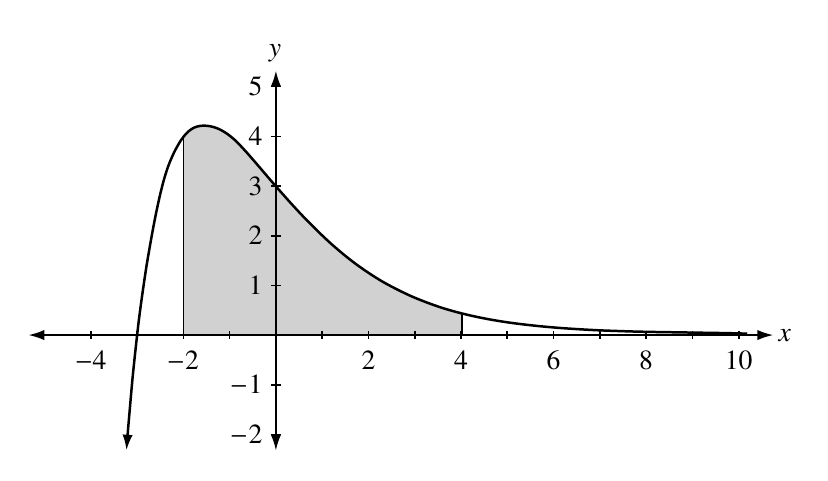
\begin{tikzpicture}[x=0.0127cm,y=-0.0127cm,font=\fontsize{10}{12}\selectfont]
  \begin{scope}\clip (174,0) rectangle (452.5,307.5);
    \fill[shade] plot[smooth]coordinates {(117,423) (118.4,404.1) (120,385.5) (121.6,367.1) (123.3,348.4) (125.2,330) (127.2,311.7) (129.3,293.3) (131.7,275) (134.3,256.7) (137,238.7) (140.1,220.5) (143.3,202.6) (146.8,184.7) (150.6,167.3) (154.6,151.6) (159.2,137.4) (164.8,124.5) (171.2,113.1) (177,105.7) (182.3,101.3) (187.3,99) (193.6,98.01) (201,98.63) (208.9,101.1) (217.2,105.8) (226,112.9) (236,123.4) (247.8,136.9) (260,151.2) (272.1,165.1) (284.2,178.6) (296.3,191.5) (308.5,203.7) (320.9,215.4) (333.7,226.4) (346.6,236.5) (359.8,245.7) (373.4,254.2) (387.8,261.9) (402.3,268.8) (417.4,274.9) (433.1,280.4) (448.7,284.9) (465,288.8) (481.7,292.1) (499,294.9) (516.3,297.1) (534.2,299) (552.1,300.5) (570.3,301.7) (588.5,302.7) (606.8,303.4) (625.5,304) (644,304.4) (662.7,304.7) (681.7,305) (700.6,305.3) (719.3,305.6) (738,306.1)} -- (738,307.5) -- (117,307.5) -- cycle;
  \end{scope}
  \draw (174,307.5)--(174,109); \draw (452.5,307.5)--(452.5,285.7);
  \draw[<->] (19,307.5)--(764,307.5);
  \draw[<->] (266.5,423)--(266.5,43);
  \foreach \i in {-4,...,10} {\ifnum\i=0\else\draw ({266.5+46.3*\i},303.5)--({266.5+46.3*\i},311.5);\fi}
  \foreach \i in {-4,-2,2,4,6,8,10} \node[below] at ({266.5+46.3*\i},313) {$\i$};
  \foreach \i in {-2,...,5} {\ifnum\i=0\else\draw (261.5,{307.5-49.7*\i})--(271.5,{307.5-49.7*\i});\node[left] at (263,{307.5-49.7*\i}) {$\i$};\fi}
  \draw[<-,line width=0.9pt] plot[smooth]coordinates {(117,423) (118.4,404.1) (120,385.5) (121.6,367.1) (123.3,348.4) (125.2,330) (127.2,311.7) (129.3,293.3) (131.7,275) (134.3,256.7) (137,238.7) (140.1,220.5) (143.3,202.6) (146.8,184.7) (150.6,167.3) (154.6,151.6) (159.2,137.4) (164.8,124.5) (171.2,113.1) (177,105.7) (182.3,101.3) (187.3,99) (193.6,98.01) (201,98.63) (208.9,101.1) (217.2,105.8) (226,112.9) (236,123.4) (247.8,136.9) (260,151.2) (272.1,165.1) (284.2,178.6) (296.3,191.5) (308.5,203.7) (320.9,215.4) (333.7,226.4) (346.6,236.5) (359.8,245.7) (373.4,254.2) (387.8,261.9) (402.3,268.8) (417.4,274.9) (433.1,280.4) (448.7,284.9) (465,288.8) (481.7,292.1) (499,294.9) (516.3,297.1) (534.2,299) (552.1,300.5) (570.3,301.7) (588.5,302.7) (606.8,303.4) (625.5,304) (644,304.4) (662.7,304.7) (681.7,305) (700.6,305.3) (719.3,305.6) (738,306.1)};
  \node at (775,308) {$x$};
  \node at (265.5,26) {$y$};
\end{tikzpicture}
\end{document}
